% AI-produced by GPT-6 Astra (OpenAI), ChatGPT Pro mode.
\section{Supports and the orthomodular law}
\label{sec:supports}

We write $x\perp y$ for the primitive \emph{internal} disjunction of
156-8 and 156-9. In the earlier theory we apply the same construction to
the explicitly specified figure-disjointness relation. These two
relations must not be identified without a hypothesis. A figure may be
finite, or belong to an explicitly chosen larger class; every assertion
below states which quantifier is intended.

\subsection{Two exact tests, including infinite ordered sets}

\begin{definition}[Known: orthoset definitions]\label{SA21-A01}
An orthoset is a set $E$ with a symmetric irreflexive relation $\perp$.
For $A\subseteq E$ put
\[
 N(A)=\{x\in E:(\forall a\in A)\ x\perp a\},\qquad
 \operatorname{cl}A=N(N(A)),\qquad
 \Sigma(E)=\{A\subseteq E:A=\operatorname{cl}A\}.
\]
We abbreviate $N(\{x\})$ to $N(x)$. Orthogonality between subsets means
orthogonality of every pair of their elements. A basis of $A$ means a
maximal, under inclusion, pairwise orthogonal subset of $A$; it need not
be finite. For a poset $L$, $N_L(A)$ denotes the points strictly
comparable with every member of $A$.
\end{definition}

\begin{proposition}[Known, with the required construction checked]\label{SA21-A02}
$\Sigma(E)$ is a complete ortholattice, with
\[
 \bigwedge_i A_i=\bigcap_i A_i,\qquad
 \bigvee_i A_i=\operatorname{cl}\Bigl(\bigcup_iA_i\Bigr),\qquad
 A^\perp=N(A),\quad 0=\varnothing,\quad1=E.
\]
For $E=\varnothing$ this is the one-element ortholattice, with $0=1$.
\end{proposition}
\begin{proof}
Symmetry gives $A\subseteq N^2(A)$ and $N^3(A)=N(A)$; thus $N^2$ is a
closure operator and $N$ is an order-reversing involution on its fixed
points. Closed sets are closed under arbitrary intersections. If
$x\in A\cap N(A)$, irreflexivity is contradicted. Consequently
$A\wedge A^\perp=0$, and the dual identity follows by applying $N$.
These formulas also prove completeness, including the empty meets and
joins. This is exactly the construction of 156-9, scans 51--53 and
78--80; compare \citet[\S2]{Jenca2022}.
\end{proof}

\begin{theorem}[Known criterion, explicitly specialized and proved]\label{SA21-A03}
Let $E$ be an arbitrary orthoset. Its support lattice is orthomodular
if and only if
\begin{equation}\label{eq:basis-test}
 \text{for every }S\subseteq E\text{ and every basis }D\subseteq N(S),
 \qquad N(D)\subseteq N(N(S)).
\end{equation}
In particular, the exact answer for the comparability disjoncteur of a
poset $L$ is the following condition expressed entirely in its order:
for every $S\subseteq L$ and every maximal chain $D$ of $N_L(S)$,
every point strictly comparable with all of $D$ is strictly comparable
with every point of $N_L(S)$.
\end{theorem}
\begin{proof}
Every closed set has the form $A=N(S)$. Condition
\eqref{eq:basis-test}, together with $D\subseteq A$, is equivalent to
$N(D)=N(A)$, or $\operatorname{cl}D=A$.
Suppose the lattice is orthomodular. For a basis $D$ of $A$, let
$B=\operatorname{cl}D\leq A$. Maximality implies
$A\cap N(D)=\varnothing$: a point in this intersection could be
adjoined to $D$. Hence $A\wedge B^\perp=0$, and the orthomodular law
gives $A=B\vee(A\wedge B^\perp)=B$.
Conversely let every basis generate its closed set. Given closed
$B\leq A$, take a basis $D$ of $B$ and extend it to a basis $H$ of $A$.
Existence and extension follow from Zorn's lemma; we work in ZFC.
For $h\in H\setminus D$ we have $h\in A\cap N(D)=A\cap B^\perp$.
Therefore
\[
 A=\operatorname{cl}H\leq B\vee(A\wedge B^\perp)\leq A.
\]
This proves the orthomodular law. In the comparability orthoset,
pairwise orthogonal subsets are exactly chains, proving the asserted
order formulation. This is Dacey's basis criterion in the form of
\citet[Theorem 3.3]{Jenca2022} and
\citet[Lemma 2.11]{PasekaVetterlein2022}; it is not Sumner's weaker
maximal-clique condition.
\end{proof}

\begin{theorem}[Proved: exact Boolean test]\label{SA21-A04}
For any orthoset $E$, finite or infinite, $\Sigma(E)$ is Boolean if and
only if
\begin{equation}\label{eq:boolean-test}
 x\not\perp y\quad\Longrightarrow\quad
 (\exists z\in E)\ N(x)\cup N(y)\subseteq N(z).
\end{equation}
The quantifier includes $x=y$. For a comparability disjoncteur this is
the required necessary and sufficient condition on the order of $L$,
using $N_L$ in place of $N$. For finite $L$, it is a direct test on
triples of points and their neighbourhoods; no lattice enumeration is
required.
\end{theorem}
\begin{proof}
The inclusion in \eqref{eq:boolean-test} says precisely
$z\in\operatorname{cl}\{x\}\cap\operatorname{cl}\{y\}$.
Moreover $x\perp y$ if and only if the two singleton closures are
orthogonal. In a Boolean algebra disjoint elements are orthogonal,
so nonorthogonality forces a nonempty intersection of these closed
sets, proving necessity.
For sufficiency, if closed $A,B$ are not orthogonal, take
$x\in A,y\in B$ with $x\not\perp y$. The specified $z$ belongs to
$A\cap B$. Thus for closed sets, zero meet implies orthogonality.
We verify the purely lattice-theoretic last step. In any ortholattice
with this property, $a\leq b$ and $b\wedge a^\perp=0$ imply
$b\leq a$; hence the lattice is orthomodular. To see this last
criterion directly, set $c=a\vee(b\wedge a^\perp)$; then
$b\wedge c^\perp=0$, so $b=c$.
Now let $d=(a\wedge c)\vee(b\wedge c)$ and
$e=(a\vee b)\wedge c$. We have $d\leq e$. Put
$t=e\wedge d^\perp$. Both $t\wedge a$ and $t\wedge b$ are zero,
so $t\leq a^\perp\wedge b^\perp=(a\vee b)^\perp$; also
$t\leq a\vee b$. Hence $t=0$, and orthomodularity gives $e=d$.
This is distributivity. The converse implication from orthogonality
to zero meet was already established in Proposition~\ref{SA21-A02}.
\end{proof}

\subsection{The interval magasin and the false Sumner equivalence}

\begin{definition}[Proved: the interval magasin]\label{SA21-A05}
For any poset $L$ let
\[
 M(L)=\{P_a:a\in L\}\amalg\{I_{ab}:a<b\text{ in }L\}.
\]
The endpoint set is $\delta(P_a)=\{a\}$ and
$\delta(I_{ab})=\{a,b\}$. The positional order is
\[
 U<_{\rm p}V\quad\Longleftrightarrow\quad
 U\ne V\ \text{ and }\ (\forall u\in\delta(U),v\in\delta(V))\ u\leq v.
\]
Primitive internal disjunction is strict comparability for this order.
Incidence has only $P_a,P_b\lhd I_{ab}$ in addition to identities.
Interior refinement, written $\rho$, has identities and
\[
 P_x\rho I_{ab}\iff a<x<b,\qquad
 I_{cd}\rho I_{ab}\iff a\leq c<d\leq b.
\]
A prefigure is a positional chain. A figure must additionally contain
the endpoints of each of its intervals. Thus a singleton interval is
a prefigure and is not a figure. These are the data of 156-8,
scans 90--127 and 156-9, scans 5--7, with the distinction required by
the latter page restored.
\end{definition}

% Insert immediately after Definition SA21-A05.
% AI-produced by GPT-6 Astra (OpenAI), ChatGPT Pro mode, 19 November 2026.
\begin{proposition}[Proved: the interval construction for every poset]
\label{SA21-A05a}
For every poset $L$, the relations of Definition~\ref{SA21-A05}
satisfy strong Mag~1--4. The magasin $M(L)$ is faithful if and only
if $L$ is a chain, including the empty and one-point cases. In the
full atlas its figures are precisely the positional chains closed
under adjoining interval endpoints. Restricting the atlas to finite
figures gives exactly the finite such chains; no local finiteness
or density of $L$ is needed.
\end{proposition}
\begin{proof}
We check the strong primed formulation in
Theorem~\ref{SA21-B-mag-equivalence}, rather than invoking an
unverified general construction. Incidence is a partial order since
its only strict relations run from a point to an interval having
that endpoint. Interior refinement $\rho$ is a partial order:
interval refinement is containment of the two ordered endpoints,
and $P_x\rho I_{cd}\rho I_{ab}$ gives
$a\le c<x<d\le b$, hence $P_x\rho I_{ab}$. The remaining
transitivity cases are identities; antisymmetry follows directly
from equality of both endpoints for mutual interval containment.

There is at most one $Z$ with $U\rho Z\le V$. This is immediate
when $V$ is a point. If $V=I_{ab}$, the only candidates are
$P_a,P_b,I_{ab}$. Refining a point internally requires equality;
neither endpoint point internally refines $I_{ab}$. Thus no two
candidates work. For exchange, let $U'\le U\rho V$. If $U'=U$
take $V'=V$. Otherwise $U=I_{cd}$, $V=I_{ab}$ with
$a\le c<d\le b$, and $U'$ is one of its endpoint points.
If that endpoint is $a$ or $b$, take the corresponding endpoint
point $V'\le V$; otherwise it lies strictly between $a,b$, so
take $V'=V$. In each case $U'\rho V'\le V$. Consequently
general refinement $U\ll V\iff\exists Z\,(U\rho Z\le V)$
has the required unique carrier and exchange calculus.

The positional relation is a strict partial order. Transitivity
follows by comparing all endpoints through the nonempty endpoint
set of the middle symbol. A putative cycle would force all these
endpoints equal, so all its symbols would be the same point,
contradicting strictness. Its comparability relation is therefore
symmetric and irreflexive. Suppose $U<_{\rm p}V$ and
$U'\rho U$, $V'\rho V$. Every endpoint of $U'$ is at most
every endpoint of $V'$, by the endpoint containment inequalities.
Equality $U'=V'$ could only be a common point at an endpoint of
one of the original intervals; such a point cannot internally
refine that interval. The alternative that both originals are
that point contradicts $U<_{\rm p}V$. Hence
$U'<_{\rm p}V'$, proving heredity of disjunction. Finally the
principal incidence ideal of $I_{ab}$ consists of
$P_a,I_{ab},P_b$, in that positional order. All three distinct
pairs are internally disjoint. Point ideals are singletons.
This is the full two-strata condition, not merely its
comparable-incidence weakening, and completes strong Mag~1--4.

The full-atlas statement follows from the clique-downset
construction in Theorem~\ref{SA21-B-mag-equivalence}: positional
cliques are chains and incidence closure is exactly endpoint
closure. Adjoining endpoints to any such chain, finite or infinite,
preserves its positional order. Indeed a symbol preceding $I_{ab}$
has every endpoint at most $a$, and one following it has every
endpoint at least $b$. Existing equal endpoint symbols are simply
identified. This also proves the stated finite-atlas description.

If $L$ is a chain, any nonorthogonal pair has a common interior
refinement. Equal points use themselves; a point nonorthogonal
to $I_{ab}$ satisfies $a<x<b$ and again uses itself. Two
nonorthogonal intervals $I_{ab},I_{cd}$ satisfy
\[
 \max(a,c)<\min(b,d),
\]
so $I_{\max(a,c),\min(b,d)}$ internally refines both. This
uses no intermediate point or density assumption. Conversely
a common interior refinement precludes orthogonality by the
heredity just proved and irreflexivity. Thus the faithfulness
equivalence holds. If $L$ is not a chain, choose incomparable
$x,y$. The symbols $P_x,P_y$ are nonorthogonal, but only $P_x$
internally refines $P_x$ and only $P_y$ internally refines $P_y$;
there is no common interior refinement. This refutes faithfulness.
The empty and singleton cases satisfy both conditions directly.
\end{proof}


\begin{theorem}[Proved: exact answers for all $M(L)$]\label{SA21-A06}
The lattice $\Sigma(M(L))$ is orthomodular exactly when the order test
of Theorem~\ref{SA21-A03} holds on the explicit positional poset in
Definition~\ref{SA21-A05}. Equivalently, for every set $S$ of points
and intervals and every maximal positional chain $D$ of those symbols
strictly comparable with all of $S$,
\[
 N_{M(L)}(D)\subseteq N_{M(L)}(N_{M(L)}(S)).
\]
It is Boolean exactly when the nonisolated points of $L$ form a chain.
Here a point is nonisolated if it is comparable with a distinct point
of $L$; all remaining points may be arbitrary isolated points.
For a nontrivial connected $L$, the Boolean condition is simply that
$L$ is a chain. No finiteness or local finiteness is assumed.
\end{theorem}
\begin{proof}
The first assertion is a direct application of Theorem~\ref{SA21-A03}
to the explicitly specified order and therefore proves both directions
without assuming the conclusion about $\Sigma$.
For the Boolean assertion first suppose that $x$ is nonisolated.
We prove $\operatorname{cl}\{P_x\}=\{P_x\}$. If $Y\ne P_x$ is
orthogonal to $P_x$, then $Y\in N(P_x)$ and $Y\notin N(Y)$ already
separates the points. Otherwise choose a neighbour $u$ of $x$ in $L$
and let $J$ be the interval with endpoints $x,u$. It belongs to
$N(P_x)$. If $Y=P_y$ and $y$ is incomparable with $x$, then
$J\not\perp P_y$, since either positional comparability would force
$x$ comparable with $y$. If $Y=I_{ab}$, nonorthogonality with $P_x$
means $x\not\leq a$ and $b\not\leq x$.
For $u>x$, $J\perp I_{ab}$ would require $u\leq a$ or $b\leq x$;
both are impossible. The case $u<x$ is dual. Thus every other $Y$ is
excluded from the singleton closure.
If $\Sigma(M(L))$ is Boolean, distinct such singleton atoms are
orthogonal, so their underlying points are comparable. This proves
necessity.
Conversely let the nonisolated core $C$ be a chain. On $M(C)$,
two symbols are not orthogonal exactly when they have a common
interior refinement: for points this is equality or strict membership
in an interval, and for two intervals the common interval or point is
obtained from their overlap. Consequently this magasin is faithful,
and Proposition~\ref{SA21-A12} identifies its support lattice with a
complete Boolean algebra of regular open sets. Adjoining isolated
points adds isolated vertices to the orthogonality graph. If $C$ is
nonempty, every proper closed set is contained in $M(C)$ and is the
same proper closed set as before; the old top is replaced by the new
top. This is an ortholattice isomorphism. If $C$ is empty and $L$ is
nonempty the graph has no edges and its lattice has two elements;
if $L$ is empty its lattice has one element. Both are Boolean.
\end{proof}

\begin{counterexample}[Refuted: L2 and global orthomodularity of $M(L)$]
\label{SA21-A07}
Let $L=\{a,b,c,d\}$ with exactly $a<c,a<d,b<c,b<d$.
Then $M(L)$ has eight strata. Its edges are the four point edges
\[
 ac,ad,bc,bd
\]
and the two endpoint edges for each of $I_{ac},I_{ad},I_{bc},I_{bd}$.
Its twenty supports are: $\varnothing$; the eight singleton sets;
the six two-element subsets of $\{P_a,P_b,P_c,P_d\}$;
the four neighbourhoods $N(P_x)$; and $M(L)$.
The strict inclusion
\[
 A=\{P_a\}<B=\{P_a,P_b\},\qquad B\cap A^\perp=\varnothing
\]
violates orthomodularity. Nevertheless every figure satisfies
Axiome supp~1, and the graph satisfies Sumner's Dacey-graph condition.
Taking the positional order itself as an eight-element poset also
refutes L2 for comparability disjoncteurs.
\end{counterexample}
\begin{proof}
The listed edges follow by substituting the four comparisons in
Definition~\ref{SA21-A05}. Intersections of their eight neighbourhoods
give exactly the twenty sets displayed; the attached exhaustive
certificate independently enumerates all $2^8$ subsets and all
ortholattice operations. The displayed $A,B$ are among those sets,
and $N(P_a)=\{P_c,P_d,I_{ac},I_{ad}\}$, proving the failure.
The maximal cliques are exactly the four triangles
$\{P_x,I_{xy},P_y\}$. If such a triangle is covered by
$N(u)\cup N(v)$, its interval vertex forces one of $u,v$ to be an
endpoint, say $u$. To cover that endpoint, $v$ must be adjacent to
$u$, since a vertex is not in its own neighbourhood. This is exactly
Sumner's condition. Theorem~\ref{SA21-A09} below proves the figure
assertion for every $L$, independently of the enumeration.
\end{proof}

\begin{theorem}[Proved: the precise meaning of Sumner's condition]
\label{SA21-A08}
For an orthoset in which all cliques are admitted as figures, the
following are equivalent:
\begin{enumerate}
\item For every clique $F$ and $A\subseteq F$,
$\operatorname{cl}F\cap N(A)=\operatorname{cl}(F\setminus A)$.
\item For every maximal clique $D$ and every distinct $u,v$,
$D\subseteq N(u)\cup N(v)$ implies $u\perp v$.
\end{enumerate}
The equivalence holds also for infinite cliques, using choice. On
finite graphs (2) is precisely \citet[p.~492]{Sumner1974}, and is
normality in the terminology of \citet[Definition 2.4 and Lemma 2.5]
{PasekaVetterlein2022}. On an infinite orthoset their normality tests
finite orthogonal families; we do not identify that convention with
an unrestricted infinite-family assertion. The finite condition is
strictly weaker than the basis criterion
of Theorem~\ref{SA21-A03}, even for finite comparability graphs.
\end{theorem}
\begin{proof}
The two-neighbourhood characterization in
Theorem~\ref{SA21-A16} proves that (1) implies (2), because a maximal
clique has empty polar and hence closure $E$.
Conversely take a clique $F$, $z\in\operatorname{cl}F$, and $w$ with
$F\subseteq N(z)\cup N(w)$. Extend $F$ to a maximal clique $D$.
Every $d\in D\setminus F$ lies in $N(F)$ and is therefore
orthogonal to $z$. Consequently $D\subseteq N(z)\cup N(w)$.
The case $z=w$ would give $z\in N(F)\cap\operatorname{cl}F$,
which is impossible. Thus (2) gives $z\perp w$, and
Theorem~\ref{SA21-A16} gives (1). Strictness is the preceding
eight-vertex example. In particular, replacing ``Dacey space'' by
``Dacey graph in Sumner's sense'' is an invalid use of the shared name.
\end{proof}

\begin{theorem}[Proved: every finite flag is admissible]
\label{SA21-A09}
Every finite prefigure, and hence every finite figure, of $M(L)$
satisfies Axiome supp~1 for every poset $L$.
This conclusion does not assert orthomodularity of the whole support
lattice, nor does it extend to arbitrary infinite figures.
\end{theorem}
\begin{proof}
The endpoints of a finite prefigure form a finite chain
$t_0<\cdots<t_n$. Inserting all points $P_{t_i}$ and all intervals
$I_{t_it_{i+1}}$ yields an alternating flag $H$ containing the
prefigure. An original interval has consecutive endpoints in this
chain: another endpoint strictly between them would be incompatible
with that interval. The empty prefigure is immediate; a one-point
flag causes no difficulty.
For a symbol $Z$ let
$T_Z=\{h\in H:Z\not\perp h\}$. If nonempty, $T_Z$ is a contiguous
block in $H$: all members before it are positionally below $Z$,
and all members after it are above $Z$, by transitivity of the
positional order. Suppose $T_Z,T_W$ are nonempty and disjoint, with
$T_Z$ before $T_W$. Choose consecutive $h_i,h_{i+1}$ at a cut between
these blocks. Then $Z<_{\rm p}h_{i+1}$ and $h_i<_{\rm p}W$.
The consecutive symbols are either $P_t,I_{tu}$ or $I_{st},P_t$.
In either case the two inequalities say that every endpoint of $Z$
is at most $t$ and every endpoint of $W$ is at least $t$. Thus
$Z<_{\rm p}W$, except possibly equality of the same point symbol,
which the disjoint nonempty traces exclude.
Now let $Z\in\operatorname{cl}H$ and
$H\subseteq N(Z)\cup N(W)$. The first trace is nonempty, since
$\operatorname{cl}H\cap N(H)=\varnothing$. The traces are disjoint.
If $T_W$ is empty, $W\in N(H)$ directly gives $Z\perp W$;
otherwise the preceding argument does. Theorem~\ref{SA21-A16}
proves admissibility of $H$. Its Boolean family of subjoins is closed
under intersections and relative complements, so restricting that
family to any subflag proves the assertion for the original
prefigure. This supplies the missing global comparison in the
finite-flag computation of 156-9, scans 21--22.
\end{proof}

\begin{counterexample}[Refuted: an unrestricted infinite extension]
\label{SA21-A10}
Let $L=\mathbb Q\amalg\{a,b\}$, with the usual order on $\mathbb Q$,
with $a<q$ exactly for $q\geq0$, and with $q<b$ exactly for $q<0$.
There are no other comparisons involving $a,b$.
The countable figure $F=\{P_q:q\in\mathbb Q\}$ of $M(L)$ violates
Axiome supp~1. Thus a statement for finite flags cannot silently be
upgraded to all figures of the maximal, infinitary magasin.
\end{counterexample}
\begin{proof}
The declared order is transitive. We have $N(F)=\varnothing$.
No rational point is orthogonal to itself; $P_a$ misses negative
rationals and $P_b$ misses nonnegative rationals. A rational-endpoint
interval contains a rational interior point to which it is not
orthogonal. An interval $I_{a,q}$ misses every negative rational,
and an interval $I_{q,b}$ misses every nonnegative rational. These
are all possible symbols. Hence $\operatorname{cl}F=M(L)$.
Put $A=\{P_q:q\geq0\}$ and $B=F\setminus A$.
Then $P_a\in N(A)$, while $P_b\in N(B)$ and $P_a\not\perp P_b$.
Consequently $P_a\notin\operatorname{cl}B$, although
$P_a\in\operatorname{cl}F\cap N(A)$.
This is an infinite counterexample proved directly; no finite search
is offered as a certificate for its infinite assertion.
\end{proof}

\subsection{The ten-element example in the original scan}

\begin{counterexample}[Proved reconstruction; refuted orthomodular law]
\label{SA21-A11}
Put $I=\{i,i',j,k\}$ and let
\[
 \mathcal T=\{E\subseteq I:(i\in E\Longleftrightarrow i'\in E)\}
       \cup\{\{i\},\{i',j,k\}\}.
\]
Ordered by inclusion, with orthocomplement $E\mapsto I\setminus E$,
$\mathcal T$ is a ten-element ortholattice and is not orthomodular.
It reconstructs the set formula of 156-9, scan 113. We assign
\[
\begin{array}{c|cccccccccc}
\text{label}&0&a'&a&b&c&A&A'&B&C&1\\ \hline
\text{set}&\varnothing&\{i\}&\{i,i'\}&\{j\}&\{k\}&
\{j,k\}&\{i',j,k\}&\{i,i',k\}&\{i,i',j\}&I
\end{array}
\]
The covers are
\[
0\prec a'\prec a,\quad0\prec b,\quad0\prec c,\quad
a\prec B,C,\quad b\prec A,C,\quad c\prec A,B,\quad
A\prec A'\prec1,\quad B,C\prec1.
\]
In particular, a transcribed edge $c\to C$ must not be included.
\end{counterexample}
\begin{figure}[htbp]
\centering
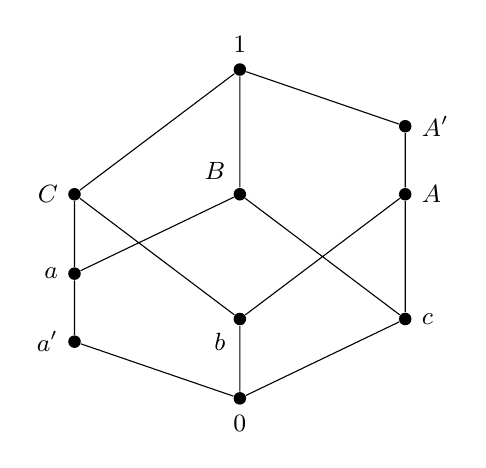
\begin{tikzpicture}[x=1.05cm,y=.72cm,
  dot/.style={circle,fill,inner sep=1.6pt},
  every label/.style={font=\small}]
\node[dot,label=below:$0$] (zero) at (0,0) {};
\node[dot,label=left:$a'$] (ap) at (-2,1) {};
\node[dot,label=left:$a$] (a) at (-2,2.2) {};
\node[dot,label=below left:$b$] (b) at (0,1.4) {};
\node[dot,label=right:$c$] (c) at (2,1.4) {};
\node[dot,label=right:$A$] (A) at (2,3.6) {};
\node[dot,label=above left:$B$] (B) at (0,3.6) {};
\node[dot,label=left:$C$] (C) at (-2,3.6) {};
\node[dot,label=right:$A'$] (Ap) at (2,4.8) {};
\node[dot,label=above:$1$] (one) at (0,5.8) {};
\draw (zero)--(ap)--(a) (zero)--(b) (zero)--(c)
 (a)--(B) (a)--(C) (b)--(A) (b)--(C)
 (c)--(A) (c)--(B) (A)--(Ap)--(one)
 (B)--(one) (C)--(one);
\end{tikzpicture}
\caption{The reconstructed ten-element ortholattice of scan 156-9/113.
Only the marked points are vertices; unmarked edge crossings are not.
The labels refer to the set table in Counterexample~\ref{SA21-A11}.}
\label{fig:ten-element}
\end{figure}
\begin{proof}
The eight sets satisfying the equivalence form an ordered Boolean
cube. Inserting $a'$ between $0,a$ and $A'$ between $A,1$ preserves
existence of binary meets and joins: for an old element $x$, the meet
with $a'$ is $a'$ if $a\leq x$ and $0$ otherwise; its join with
$a'$ is $a'$ if $x=0$, and otherwise the old join $a\vee x$ unless
$x\geq a$, in which case it is $x$. The dual formulas apply to $A'$.
Finally $a'\wedge A'=0$ and $a'\vee A'=1$. These formulas exhaust
the newly introduced pairs. Set complementation interchanges
$a',A'$ and the old complementary pairs, reverses the order, and
has zero meet and unit join on every such pair. Thus it is an
orthocomplementation.
But $a'<a$ and $a\wedge(a')^\perp=a\wedge A'=0$, refuting
orthomodularity. The program checks all 100 pairs and all required
identities. We inspected the original set formula and drawing, not
only the transcription: the second condition in the formula concerns
$i,i'$ both being outside $E$, not $j,i'$. The drawing contains
overwritten construction strokes; the set formula and valid cover
relation above provide the unambiguous mathematical reconstruction.
The lower-right handwritten label has an ambiguous extra stroke;
renaming that vertex $b$ has no mathematical effect.
The transcription also renders the powerset glyph as
$\mathcal P^3(I)$ (line 104). Our ten-element reconstruction uses
$\mathcal P(I)$. If the apparent superscript is instead read literally
as the family of three-element subsets, the displayed predicate selects
only $\{i,i',j\}$, $\{i,i',k\}$, and $\{i',j,k\}$.
They are three incomparable sets, with neither a bottom nor a top;
that reading does not define an ortholattice and cannot have cardinality
ten. The mathematical consequences of these two readings are therefore
distinct, and only the ordinary powerset reading reconstructs the
announced example.
\end{proof}

\subsection{Faithfulness, lieux, and general magasins}

\begin{proposition}[Proved: the faithful case, R1 rechecked]
\label{SA21-A12}
Let $(M,\rho,\perp)$ be a magasin whose interior refinement $\rho$ is
a preorder and whose faithfulness means
\[
 x\perp y\quad\Longleftrightarrow\quad
 \text{there is no }z\text{ with }z\rho x\text{ and }z\rho y.
\]
In the Alexandrov topology of $\rho$-lower sets,
$\Sigma(M)$ is exactly the complete Boolean algebra of regular open
sets. In particular every family of mutually orthogonal supports
satisfies the relative-complement and nonempty-meet conclusions of
the support theorem.
\end{proposition}
\begin{proof}
For $A\subseteq M$ put $O_A=\bigcup_{a\in A}\mathord\downarrow_\rho a$.
Faithfulness says
\[
 N(A)=\operatorname{int}(M\setminus O_A).
\]
Indeed a point belongs to the right side exactly when its principal
lower set meets no principal lower set of a member of $A$.
Since $N(A)$ is open, applying this formula twice gives
$\operatorname{cl}A=\operatorname{int}\overline{O_A}$.
Every such set is regular open; conversely, for a regular open set
$U$, $O_U=U$ and $\operatorname{cl}U=U$. Complement, joins and meets
are consequently the usual regular-open operations. To check the
Boolean assertion without any separation hypothesis on the topology,
if two regular opens have empty intersection, each is contained in
the interior of the complement of the other. Proposition
\ref{SA21-A04}'s lattice argument proves distributivity. In an
Alexandrov topology arbitrary intersections of opens are open; the
intersection of regular opens is regular by monotonicity of
$\operatorname{int}\overline{(-)}$, so the complete meet is their
intersection, as required by the polarity construction.
\end{proof}

\begin{theorem}[Proved: the exact general class under Mag L2]
\label{SA21-A13}
Assume the strong Mag~1--4, divisibility, and the lieu-detection
axiom Mag~L2. Let $L$ be the set of lieux and
$U_X=\{p\in L:p\rho X\}$. In this notation Mag~L2 says
\[
 X\perp Y\iff U_X\perp U_Y.
\]
The maps
\[
 \Sigma(M)\longrightarrow\Sigma(L),\ S\longmapsto S\cap L,
 \qquad
 \Sigma(L)\longrightarrow\Sigma(M),\
 T\longmapsto\widehat T=\{X:U_X\subseteq T\}
\]
are inverse complete ortholattice isomorphisms. Thus the exact class
asked for in A.2 consists of those magasins whose lieu graph satisfies
\eqref{eq:basis-test}. Their Boolean subclass is given exactly by
\eqref{eq:boolean-test} on that graph. Every orthoset occurs as the
lieu graph of a magasin satisfying these hypotheses.
\end{theorem}
\begin{proof}
The axiom forces $U_X\ne\varnothing$, since otherwise it would imply
$X\perp X$. For a lieu $p$, $U_p=\{p\}$.
For any $A\subseteq M$ write $u(A)=\bigcup_{X\in A}U_X$.
The detection formula gives
\[
 N_M(A)=\widehat{N_L(u(A))}.
\]
For any $B\subseteq L$, monotonicity of orthogonality under interior
refinement and the same detection formula give
$N_M(B)\cap L=N_L(B)$ and
$N_M(B)=\widehat{N_L(B)}$.
If $S=N_M(A)$, these identities show
$S=\widehat{S\cap L}$ and $S\cap L$ is closed in $L$.
Conversely, if $T$ is closed in $L$,
$\widehat T=N_M(N_L(T))$ is closed in $M$, and
$\widehat T\cap L=T$. The formulas also show that polars are
preserved, hence all lattice operations are preserved.
To realize an arbitrary orthoset take $M=L=E$, incidence and interior
refinement both identity, and the prescribed orthogonality. The
strong incidence-disjunction condition is vacuous beyond distinct
elements of a singleton principal ideal, and the lifting and
monotonicity axioms are identities. All vertices are lieux and
$U_x=\{x\}$, so divisibility and detection hold. Figures are the
cliques. There is consequently no further hidden restriction on
the class of possible lieu graphs.
\end{proof}

\begin{theorem}[Proved: exact answer to the atom question]
\label{SA21-A14}
In any atelier with the specified orthogonality relation, the nonzero
support $\operatorname{cl}\{x\}$ of a lieu $x$ is an atom if and only if
\begin{equation}\label{eq:atom-test}
 N(x)\subseteq N(y)\quad\Longrightarrow\quad N(x)=N(y)
 \qquad (y\in M).
\end{equation}
Under the hypotheses of Theorem~\ref{SA21-A13}, it suffices to test
$y\in L$. Hence the exact class in A.3 is given by
\eqref{eq:atom-test} for every lieu. The stronger assertion that
$\operatorname{cl}\{x\}=\{x\}$ requires
$N(x)\subseteq N(y)\Rightarrow y=x$ and is different.
\end{theorem}
\begin{proof}
The inclusion of neighbourhoods is equivalent to
$\operatorname{cl}\{y\}\subseteq\operatorname{cl}\{x\}$.
Every nonempty closed set contains the nonempty closure of any one of
its points. Minimality of $\operatorname{cl}\{x\}$ is therefore
equivalent to equality of these singleton closures whenever they
are included. Applying $N$ translates that equality into
\eqref{eq:atom-test}. Under lieu detection, every nonzero closed set
contains a lieu, by the isomorphism and nonemptiness of the $U_X$.
The same proof then restricts the test to lieux. The stronger
singleton statement follows directly from
$y\in\operatorname{cl}\{x\}\iff N(x)\subseteq N(y)$.
\end{proof}

% Insert after Theorem SA21-A14 and its proof.
% AI-produced by GPT-6 Astra (OpenAI), ChatGPT Pro mode, 19 November 2026.
\begin{corollary}[Proved: the exact atom class for interval magasins]
\label{SA21-A14a}
For every poset $L$, the lieux of $M(L)$ are exactly the point symbols
$P_x$. All these lieux have atomic supports if and only if $L$ is an
antichain or $L$ has no isolated points. Thus every lieu has an atomic
support for every nonempty connected poset, including the singleton.
For $L=\varnothing$ the assertion is vacuous.
\end{corollary}
\begin{proof}
We use the manuscript's full-refinement definition of a lieu:
minimality for $\ll$, not merely for interior refinement $\rho$
(156-8, scan~15, \path{J156-8-02_transcription.tex:277}).
In the primed formulation it is minimality for both incidence and
$\rho$ (\path{J156-8-04_transcription.tex:282,296}).
Only $P_x$ refines $P_x$, since a factorization
$U\rho Z\le P_x$ forces $Z=P_x$ and then $U=P_x$.
Every interval $I_{ab}$ has the distinct incidence predecessor
$P_a$, which also refines it. Thus the lieux are exactly the points,
even when $a\lessdot b$ makes $I_{ab}$ minimal for $\rho$ alone.
In particular we make no unsupported divisibility claim for intervals
having no point strictly between their endpoints.

Theorem~\ref{SA21-A06} proves that every nonisolated $x$ has
$\operatorname{cl}\{P_x\}=\{P_x\}$, a nonzero atom.
For an isolated $x$, the symbol $P_x$ has no neighbour, so
$\operatorname{cl}\{P_x\}=M(L)$. If $L$ has a comparison $a<b$,
the singleton support of $P_a$ is a proper nonzero closed set,
and this top support is not an atom. If $L$ is a nonempty antichain,
there are no interval symbols and no disjunction edges; its support
lattice has just zero and one, so every lieu has that single nonzero
atom as support. These alternatives prove both directions of the
criterion. A connected comparability graph with more than one vertex
has no isolated point, and the singleton case is an antichain.
The empty case follows from the universal quantifier over no lieux.
\end{proof}


\begin{counterexample}[Refuted inference; R2 and L3 precisely qualified]
\label{SA21-A15}
Two lieux with no edge have the two-element Boolean support lattice;
their supports are the same atom. Thus nondisjoint distinct lieux do
not, by themselves, measure failure of distributivity. Under Mag~L2
and divisibility, the following are equivalent: faithfulness;
Booleanity with lieux represented by distinct atoms; and
$p\perp q$ for every pair of distinct lieux. In the additional
point-separating case $\operatorname{cl}\{p\}=\{p\}$ for all lieux,
Booleanity alone is equivalent to pairwise disjointness of distinct
lieux. Without point separation the exact replacement is
Theorem~\ref{SA21-A04}.
For interval magasins the exact replacement is the nonisolated-core
criterion of Theorem~\ref{SA21-A06}. In particular, for a connected
poset $L$, Booleanity of $\Sigma_{M(L)}$ is equivalent to totality
of $L$, hence to disjointness of distinct lieux. Thus this precise
connected interpretation of the qualitative claim in L3 is true.
The unqualified claim fails even in a divisible interval magasin
with genuine interval strata: take $L=\mathbb Q\amalg\{c\}$,
with $c$ incomparable to every rational.
\end{counterexample}
\begin{proof}
The two-vertex graph has $N(\varnothing)=L$ and $N(A)=\varnothing$
for every nonempty $A$, proving the first claim and also showing why
the atom question is weaker than separation.
Faithfulness on distinct lieux forces orthogonality, since they have
no common interior lower bound. Conversely if distinct lieux are
orthogonal, detection says $X\not\perp Y$ precisely when
$U_X\cap U_Y\ne\varnothing$. This is equivalent to a common
interior refinement: a common lieu is one, and any common refinement
contains a lieu. Thus the magasin is faithful. Its support lattice
is $\mathscr P(L)$ under Theorem~\ref{SA21-A13}, with distinct
singleton atoms. Conversely distinct atoms of a Boolean algebra are
orthogonal, so the corresponding lieux are orthogonal. The same
argument proves the last assertion when singleton separation is
assumed. The four-lieu graph consisting of two disjoint edges gives
$MO_2$: its supports are zero, the four singletons, and one; it is
orthomodular but not distributive. This is also checked in the code.

For the connected assertion, a connected comparability graph with
at least two vertices has no isolated vertex, so its nonisolated
core is all of $L$. The empty and singleton cases cause no exception.
Apply Theorem~\ref{SA21-A06}; the lieux of an interval magasin are
its point symbols, whose disjunction is strict comparability.

For the final example the nonisolated core is the chain $\mathbb Q$,
so Theorem~\ref{SA21-A06} proves Booleanity. Every interval $I_{ab}$
has nonempty open-lieu set $\{P_q:a<q<b\}$, by density of
$\mathbb Q$, and point symbols have singleton open-lieu sets.
Two rational interval interiors are disjoint precisely when their
endpoints are positionally ordered; a rational point is orthogonal to an
interval precisely when it is outside that interval's open interior.
Together with the singleton tests this proves Mag~L2 and divisibility.
The extra lieu $P_c$ is orthogonal to no symbol, and each other open
lieu set is nonempty, so the same detection test also holds for every
pair involving it. Nevertheless $P_c\not\perp P_q$ for all rational
$q$. Its singleton support is the top, since $N(P_c)=\varnothing$.
This gives the asserted failure inside the interval construction
itself, and explains why point separation is the missing hypothesis.
\end{proof}

\subsection{The exact support theorem and the distinction from orthomodularity}

\begin{theorem}[Proved: complete characterization of A.4]
\label{SA21-A16}
Fix an orthoset $E$ and a family $(U_i)_{i\in I}$ of nonempty mutually
orthogonal subsets. Put $e_i=\operatorname{cl}U_i$,
$S_A=\operatorname{cl}(\bigcup_{i\in A}U_i)$ for $A\subseteq I$,
and $S=S_I$. The map $A\mapsto S_A$ is always an injective order map
preserving arbitrary joins. The following explicit condition is
necessary and sufficient for the remaining lattice conclusions
(a)--(c) of the Théorème of 156-7, scan 94:
\begin{equation}\label{eq:figure-test}
\begin{gathered}
 z\in S,\quad w\in E,\quad
 (\forall i\in I)\ [z\perp U_i\ \text{or}\ w\perp U_i]
 \quad\Longrightarrow\quad z\perp w.
\end{gathered}
\end{equation}
More precisely this is equivalent to all identities
\[
 S_A\cap N\Bigl(\bigcup_{i\in B}U_i\Bigr)=S_{A\setminus B}
 \qquad(B\subseteq A\subseteq I),
\]
and it implies preservation of arbitrary nonempty meets. Empty meets
are preserved into the interval $[0,S]$; they are preserved into the
whole lattice only when $S=1$.
For the atelier specialization take $I=\widetilde F$ for an admitted
figure $F$, and $E=M$ with the \emph{old
whole-figure disjunction} $\parallel$, and write $N_\parallel$
for its polar. Here $U_X$ are the actual open-stratum subsets used
to define $S_A$, or subsets with the same polars as justified below.
For every incidence-closed subfigure $G\leq F$, clause (d) has the
additional exact criterion
\begin{equation}\label{eq:incidence-coverage}
 N_\parallel(\widetilde G)
 =N_\parallel\Bigl(\bigcup_{X\in\widetilde G}U_X\Bigr).
\end{equation}
Here $\operatorname{Supp}(G)=N_\parallel^2(\widetilde G)$.
Under the older hypotheses of scan 94, nonemptiness, mutual
orthogonality and \eqref{eq:incidence-coverage} are automatic;
the exact class asked for in A.4 is then given by
\eqref{eq:figure-test} for every admitted figure. If those hypotheses
are dropped, include all three of these requirements explicitly.
Injectivity forces nonemptiness, and the relative-complement formula
for two different indices forces orthogonality. This formulation
applies to infinite figures and infinite families.
\end{theorem}
\begin{proof}
Joins are preserved by idempotence of closure. If $i\in A\setminus B$,
then $0\ne e_i\leq S_A$ and $e_i\perp S_B$, so $S_A\not\leq S_B$.
This proves order reflection and injectivity.
Assume \eqref{eq:figure-test}. If
$z\in S\cap N(\bigcup_{i\in A}U_i)$, and
$w\in N(\bigcup_{i\notin A}U_i)$, its hypothesis holds for every
$i$, so $z\perp w$. Thus $z\in S_{I\setminus A}$. The reverse
inclusion follows from mutual orthogonality and monotonicity.
Conversely, assume this relative-complement identity for every $A$.
Given the hypothesis of \eqref{eq:figure-test}, choose
$A=\{i:z\perp U_i\}$. Then $w$ is orthogonal to all $U_i$ outside
$A$, while $z\in S\cap N(\bigcup_{i\in A}U_i)=S_{I\setminus A}$;
hence $z\perp w$.
It remains to prove that the single-top identity gives all the stated
operations. Write $c_S(T)=S\cap T^\perp$. On the image of our map it
is the involution $S_A\mapsto S_{I\setminus A}$. Therefore, for a
nonempty family $(A_j)$,
\[
\begin{split}
 \bigcap_j S_{A_j}
 &=S\cap\bigcap_j S_{I\setminus A_j}^{\perp}
 =S\cap\Bigl(\bigvee_j S_{I\setminus A_j}\Bigr)^\perp\\
 &=S\cap S_{\bigcup_j(I\setminus A_j)}^\perp
 =S_{\bigcap_j A_j}.
\end{split}
\]
Intersecting $S_A$ with $S\cap S_B^\perp=S_{I\setminus B}$ gives
the full relative-complement formula. The case of the empty family
has meet $S$ in $[0,S]$ and meet $1$ in the ambient lattice, proving
the necessary edge-case qualification.

We verify clause (d) and the comparison with the manuscript's open
sets, instead of silently substituting lieux for strata. Write
$\ell(X)=\{p:p\text{ is a lieu and }p\ll X\}$ and
$V_X=\ell(X)\setminus\ell(\partial X)$. At scan 90 the open
representative is
\[
 X^\circ=\{Y\in M:Y\ll X,\ Y\parallel\partial X\}.
\]
The old L3 and L2 imply $V_X\subseteq X^\circ$. If
$Y\in X^\circ$, then $\ell(Y)\subseteq\ell(X)$ and no lieu
of $Y$ belongs to $\ell(\partial X)$, since such a lieu would
be disjoint from itself. Thus $\ell(Y)\subseteq V_X$.
Testing disjunction using old L2 now gives
$N_\parallel(X^\circ)=N_\parallel(V_X)$, so both choices give
exactly the support map stated at scans 93--94.
The earlier scan-87 definition is
$\operatorname{Supp}(X)\cap N_\parallel(\partial X)$.
Old absorption At supp~1 puts its members among refinements of $X$;
the reverse inclusion for the scan-90 representative follows from
hereditary disjointness, which gives
$Y\ll X\Rightarrow Y\in\operatorname{Supp}(X)$.
Hence those two open-set definitions agree under the hypotheses
being used here.

Finally, carriers give
$\ell(G)=\bigcup_{X\in\widetilde G}V_X$. For any $Z\in M$,
old L2 says that $Z\parallel G$ exactly when every lieu of $Z$
is disjoint from every lieu of $G$. Substituting this union and
applying L2 to $Z$ and each singleton lieu gives exactly
\eqref{eq:incidence-coverage}, for $U_X=V_X$ and therefore also
for $U_X=X^\circ$. Applying the polar once more proves
$S_{\widetilde G}=\operatorname{Supp}(G)$, clause (d).
Without the older hypotheses, equality of these two closed sets
is equivalent to equality of their polars, so the displayed
additional criterion is both necessary and sufficient. Empty $G$
is included, since both unions are empty.
\end{proof}

\begin{theorem}[Proved: the exact relation with orthomodularity]
\label{SA21-A17}
In a complete orthomodular lattice, every mutually orthogonal family
of nonzero elements satisfies the lattice clauses (a)--(c) of
Theorem~\ref{SA21-A16}. Conversely, if the relative-complement formula
holds for every two-element orthogonal family of nonzero lattice
elements, the lattice is orthomodular. Thus 156-9, scan 117, applied
to the universal spatial figures of a spatios, is equivalent to
orthomodularity. The axiom for the actual figures of a given magasin
is weaker, even under Mag~1--4, divisibility and Mag~L2.
\end{theorem}
\begin{proof}
For orthogonal $u,v$ in an orthomodular lattice the dual
orthomodular law gives
$(u\vee v)\wedge u^\perp=v$. For any subset $A$ of an orthogonal
family, let $u=\bigvee_{i\in A}e_i$ and
$v=\bigvee_{i\notin A}e_i$. Completeness and order reversal of
orthocomplement give $u\perp v$; the displayed identity gives the
relative-complement formula for $S_I=u\vee v$. This argument treats
infinite families directly. Theorem~\ref{SA21-A16} supplies the other
lattice conclusions. It is also a direct form of the commuting-element
calculus usually derived from the Foulis--Holland theorem.
Conversely, for $a\leq b$ apply the assumed identity to
$u=b^\perp$ and $v=a$; zero terms may be omitted. It yields
$(b^\perp\vee a)\wedge b=a$. Taking orthocomplements gives
$a^\perp=(b\wedge a^\perp)\vee b^\perp$, the orthomodular law
for $b^\perp\leq a^\perp$. Thus it holds for every comparable pair.
For strictness, use the graph of Counterexample~\ref{SA21-A07} with
identity incidence and identity interior refinement, so all eight
vertices are lieux. Theorem~\ref{SA21-A13} verifies every magasin
hypothesis. Theorem~\ref{SA21-A08} proves Axiome supp~1 for every
figure, whereas its twenty-element support lattice is not
orthomodular. Actual figures do not realize every orthogonal pair of
abstract supports, which is exactly the missing quantifier.
\end{proof}

\begin{counterexample}[Refuted: the disjunctive-magma support axiom]
\label{SA21-A18}
Take four lieux $a',a,b,b'$ with identity incidence and interior
refinement and only the edges $a'a,ab,bb'$.
Then every strong Mag axiom, divisibility and Mag~L2 hold, but
Axiome supp~1 fails for $F=\{a,b\}$:
\[
 \operatorname{cl}F=E,\qquad
 \operatorname{cl}F\cap N(a)=\{a',b\}\ne\{b\}
     =\operatorname{cl}\{b\}.
\]
Its support lattice is $O_6$. If ``disjunctive'' is given the stronger
spatial interpretation in which interior refinement is reconstructed
from supports, use instead the five-cycle with identity incidence
and interior refinement: its singleton supports are singletons, so
that reconstruction is identity, and the same axiom fails. Thus
both readings of the request after the marginal ``Oui!'' of 156-8,
scan 89, have an explicit counterexample.
\end{counterexample}
\begin{proof}
The identity-incidence construction was verified in
Theorem~\ref{SA21-A13}. The six closed sets are
$\varnothing,\{a\},\{b\},\{a,b'\},\{a',b\},E$.
The neighbourhood calculation proves the displayed failure, and
their inclusion order is the six-element ortholattice hexagon.
For the five-cycle the calculation is in
Counterexample~\ref{SA21-A19}. The attached code checks every subset
and every finite axiom for both examples.
\end{proof}

\begin{counterexample}[Refuted under the older hypotheses as well]
\label{SA21-A19}
The five-cycle with identity incidence and refinement is an atelier
satisfying the older At~1--7, At~L1--L3, CL(spac), At~D, At~supp and
the old absorption axiom At~supp~1 of 156-7, scan 87. Nevertheless
the relative-complement conclusion of scan 94 fails, so the theorem
as a whole is false under its stated hypotheses.
\end{counterexample}
\begin{proof}
Every vertex is a lieu, every point closure is a singleton, and the
figures are the empty set, the five vertices and the five edges.
Compatibility is clique-union, figure incidence and refinement are
inclusion. The elementary figures are singletons. This explicitly
gives At~1--7, the lifting and decomposition requirements, and
At~L1--L3. Local compatibility and disjunction are exactly their
pointwise tests, so CL(spac) and At~D hold. If $G\ll X$ with $X$
elementary, either $G=X$, when the support-separation premise is
false, or $G=\varnothing$, when $X$ itself is the required witness;
this verifies old At~supp. Finally $X^\circ=\operatorname{cl}\{X\}
=\{X\}$ proves the old absorption axiom.
Number the cycle modulo five and take $F=\{0,1\}$. Then
$\operatorname{cl}F=E$ and
$E\cap N(0)=\{1,4\}\ne\{1\}=\operatorname{cl}\{1\}$.
For meet preservation it is essential that the indexing members
belong to one figure: in this edge figure,
$S_{\{0\}}\cap S_{\{1\}}=0$ does hold, so this particular
counterexample establishes the complement failure alone. No claim
about meets is inferred merely from this calculation; the original
eight-stratum example is treated separately below.
\end{proof}

\subsection{A faithful support function that is not fully faithful}

\begin{counterexample}[Proved: answer to A.5]\label{SA21-A20}
Let $M=\{a,b\}$, with identity incidence, interior refinement
$a\rho b$ in addition to identities, and no internal disjunction.
The figures are $\varnothing,\{a\},\{b\}$.
Let $P=\{p,q\}$ and define the external support function
\[
 |a|=\{p\},\qquad |b|=\{p,q\}.
\]
It is faithful and normalized, but not fully faithful in the exact
sense of 156-8, scan 86.
\end{counterexample}
\begin{proof}
Interior refinement is a partial order. Incidence lifting is trivial;
orthogonality monotonicity and the strong incidence axiom are
vacuous. Both principal interior lower sets contain $a$, so the
magasin itself is faithful. Since incidence is identity, external
open and full supports coincide. They are nonempty, monotone under
interior refinement, and their intersections are always nonempty.
Thus they detect exactly the prescribed empty disjunction relation.
They cover $P$ and distinguish its two points, satisfying the usual
normalization and separation conventions as well.
Full faithfulness requires, for a figure $F$,
\[
 \bigcup_{Z\perp F}|Z|^\circ=P\setminus|F|.
\]
For $F=\{a\}$ the left side is empty, while the right side is
$\{q\}$. Hence full faithfulness fails. This property is not
equivalent to reflecting refinement, and a constant singleton
support function would not provide the required counterexample.
\end{proof}

\subsection{Spatios, disjoncteurs, and their actual morphisms}

\begin{theorem}[Proved: the object dictionary and its zero convention]
\label{SA21-A21}
A spatios satisfying Spat~1--3 of 156-9, scans 51--53 and 78--80,
is exactly a complete ortholattice. For a complete ortholattice $K$,
put $E_K=K\setminus\{0\}$ and $x\perp y\iff x\leq y^\perp$.
Then
\[
 K\longrightarrow\Sigma(E_K),\quad
 s\longmapsto\{x\ne0:x\leq s\}
\]
is a complete ortholattice isomorphism. If zero is retained, the
relation is not irreflexive; the manuscript allows a self-orthogonal
point only when it is orthogonal to every point. Removing this
radical is the exact comparison with ordinary orthosets.
\end{theorem}
\begin{proof}
Spat~1 is completeness of the order, Spat~2 is an order-reversing
involution, and Spat~3 is the zero-meet complement identity; the
unit-join identity follows by the involution. These are precisely
the stated ortholattice axioms. For $A\subseteq E_K$, its polar is
the nonzero principal ideal below $(\bigvee A)^\perp$, and its
double polar is the nonzero principal ideal below $\bigvee A$.
All such ideals occur, and inclusion and complement give the claimed
isomorphism. If a symmetric relation has radical $R$ consisting of
its self-orthogonal points and each such point is universally
orthogonal, every closed set contains $R$. Removing $R$ and adding
it back are inverse isomorphisms of the resulting support lattices.
The empty orthoset represents the one-element spatios.
\end{proof}

\begin{theorem}[Proved: the correspondence category; L7 corrected]
\label{SA21-A22}
Let $E,F$ be orthosets. A saturated correspondence of the final
156-9 construction is a map $\alpha:E\to\Sigma(F)$ such that
\begin{equation}\label{eq:bond}
 x\in\operatorname{cl}_E A\quad\Longrightarrow\quad
 \alpha(x)\subseteq\bigvee_{a\in A}\alpha(a)
 \qquad(A\subseteq E).
\end{equation}
It corresponds bijectively to a complete join-preserving map
$f:\Sigma(E)\to\Sigma(F)$ by
\[
 f(S)=\bigvee_{x\in S}\alpha(x),\qquad
 \alpha(x)=f(\operatorname{cl}_E\{x\}).
\]
Composition is
$(\beta\alpha)(x)=\bigvee_{y\in\alpha(x)}\beta(y)$ and the identity
is $x\mapsto\operatorname{cl}\{x\}$.
If $g$ is the order right adjoint of $f$, the transposed
correspondence induces
$f^\dagger=C_EgC_F$, characterized by
\[
 f(S)\perp T\quad\Longleftrightarrow\quad S\perp f^\dagger(T).
\]
Consequently orthosets with these correspondences are equivalent
as a category to complete ortholattices with all complete join maps.
They are not the category of orthosets with ordinary functions
preserving orthogonality. L7 is false with that unqualified morphism
claim and true only with this explicit object and arrow dictionary.
\end{theorem}
\begin{proof}
If $f$ preserves all joins, including the empty join, the displayed
definition of $\alpha$ gives \eqref{eq:bond}, because
$\operatorname{cl}A=\bigvee_{a\in A}\operatorname{cl}\{a\}$.
Conversely, \eqref{eq:bond} implies
$\bigvee_{x\in\operatorname{cl}A}\alpha(x)=
\bigvee_{a\in A}\alpha(a)$, so the stated $f$ preserves joins.
Putting $A=\{x\}$ and using $x\in\operatorname{cl}\{x\}$ proves
that the two assignments are inverse. The composition and identity
formulas follow by substituting these expressions and associating
joins.
The right adjoint exists for any complete join map and is
$g(T)=\bigvee\{S:f(S)\leq T\}$. Therefore
\[
 f(S)\leq C_FT\iff S\leq g(C_FT)
       \iff S\perp C_Eg(C_FT).
\]
Since $g$ preserves meets, $C_EgC_F$ preserves joins. The displayed
adjunction characterizes it uniquely, proves involutivity of the
dagger and reverses composition. Equivalently,
\eqref{eq:bond} says that for every $y\in F$ the column
$\{x:\alpha(x)\perp y\}$ is closed: either implication follows
by applying the respective closure condition to that column.
This is the two-sided saturation of the relation in 156-9,
scans 95--100. The object functor is essentially surjective by
Theorem~\ref{SA21-A21}, and the arrow bijection is full and faithful,
which proves the claimed categorical equivalence.
For the failure of the ordinary-function interpretation, take
classical orthosets, with $x\perp y\iff x\ne y$.
Their support lattices are powersets and every relation gives a
complete join map. A relation sending one point to two points is
not a function. A relation sending two distinct points to the same
point is a function but does not preserve orthogonality. Both are
saturated correspondences. The finite certificate includes these
two examples. Earlier uses of the word ``morphism'' in the notes
have different extra requirements and are not silently identified
with this final correspondence category.
\end{proof}

\begin{theorem}[Proved: the typed spatial reconstruction]
\label{SA21-A23}
Let $(E,\preceq,\perp)$ have a partial incidence order and an
orthoset relation. For each $x$ label its principal incidence ideal
by $y\mapsto\operatorname{cl}\{y\}$, transporting the incidence
order. Assume that these labels form an elementary ordered spatial
figure: the labels are nonzero, distinct, and pairwise orthogonal.
Assume also that the resulting ordered deployment $D_x$ determines
$x$ injectively. There is then a unique spatial interior refinement
making these data a strong magasin. It is given by the existence
of an order-preserving carrier
\[
 h:D_x\longrightarrow D_y,\qquad S\subseteq h(S),
 \qquad h(\operatorname{cl}\{x\})=\operatorname{cl}\{y\}.
\]
This is the fully typed interpretation of At~spat~1--3 in 156-9,
scan 50, using the spatial target explicitly defined on scan 48.
If that target is read merely as disjoint subsets of $E$, the
assertion is false and strong At~4 must be added.
\end{theorem}
\begin{proof}
The carrier, when it exists, is unique: a nonzero closed set cannot
lie below two different orthogonal labels in $D_y$. Identities and
composition prove reflexivity and transitivity. If carriers exist
in both directions, their composites send each label $S$ to a label
$U$ of the same deployment with $S\subseteq U$. Distinct labels
there are orthogonal, so $S=U$; the intermediate inclusion is also
equality. The deployments and their transported orders coincide,
and injectivity gives $x=y$. Thus the relation is a partial order.
If $z\preceq x$, restricting a carrier to $D_z$ lands in the
principal ideal below its value on the top label of $D_z$; that ideal
is the deployment of the corresponding stratum of $y$. This proves
incidence lifting and uniqueness. Allowing a carrier without the
top-preserving condition gives exactly its composite with incidence:
factor through the principal ideal below the top image. Internal
orthogonality is monotone because the top labels are included, and
two distinct strata under one incidence top are orthogonal by the
typed deployment hypothesis. These are strong Mag~1--4. The
carrier description is precisely the sufficient ``Raff'' condition
defining spatiality on scans 46--47, and it also proves uniqueness.
For the weaker interpretation use the five-cycle orthoset with
incidence $0,2\prec1$ and all other incidences identities. Its
singleton closures are singletons. All deployments are distinct
ordered families of disjoint nonempty subsets, and comparable
distinct strata are orthogonal. But the two strata $0,2$ below $1$
are not orthogonal, violating strong At~4. This finite example is
checked by the program. Scan 47's margin and scan 49 explicitly
retain At~4, consistent with the corrected typed formulation.
\end{proof}

\begin{counterexample}[Proved: R5's simultaneous failures rechecked]
\label{SA21-A24}
The supplied eight-stratum example satisfies its stated older
hypotheses, and both nonempty-meet preservation and relative
complementation fail in one figure. Its complete data are
\[
 M=\{a,b,X,p,e,w,h,g\},\qquad a,b\lhd X,\quad p\rho X,
\]
with no other nonidentity generating incidences or interior
refinements. The lieu graph on $\{a,b,p,e,w,h,g\}$ has edges
\[
 ab,ap,bp,ae,bw,pw,eh,hg,gw.
\]
Internal disjunction adds $Xa,Xb,Xw$. Old full figure-disjointness
has the displayed lieu edges and no edge at $X$.
\end{counterexample}
\begin{proof}
The only nontrivial principal incidence figure is $\{a,b,X\}$;
its three strata are internally orthogonal. Interior refinement
has the sole nonidentity relation $p\rho X$, and the neighbours
of $X$ are exactly those of $p$, proving monotonicity. Incidence
lifting for $p\rho X$ is immediate, since $p$ has no proper face.
Every stratum has a lieu in its open shadow. Detection by lieu
shadows holds by the specified edges, and compatibility and full
disjunction are the corresponding pairwise tests on the principal
figures. This proves strong Mag~1--4 and the older L1--L3 and
CL(spac), which imply the older relative C and D conditions by the
carrier construction. For completeness the program enumerates all
figures, all their restrictions, and every instance of the older
support-separation axiom; all pass.
The full-disjunction singleton closures of the seven lieux are
singletons. The full support of $X$ is $M$, and
$X^\circ=M\cap N(\{a,b\})=\{p\}$; thus old absorption holds for
every multistrate. In the figure $F=\{a,b,X\}$ the open strata are
$\{a\},\{b\},\{p\}$. Direct intersections of neighbourhoods give
\[
\begin{aligned}
 S_F\cap S_a^\perp&=\{b,p,e\},& S_{\{b,X\}}&=\{b,p\},\\
 S_{\{a,X\}}\cap S_{\{a,b\}}&=\{a,w\},&S_{\{a\}}&=\{a\}.
\end{aligned}
\]
Both inequalities are strict. The certificate lists all eighteen
closed sets for the full-disjunction graph, the open parts of all
eight multistrates, all axiom flags, and the displayed witnesses.
This rechecks SA21-K7b-15 and SA21-R7b-21 rather than inferring them
from the smaller five-cycle example.
\end{proof}

\begin{proposition}[Proved: the cograph sufficient condition is strict]
\label{SA21-A25}
Every finite cograph has an orthomodular support lattice. The converse
fails even for a five-element comparability poset with a Boolean
support lattice.
\end{proposition}
\begin{proof}
We use the recursive definition of cographs: start with one vertex
and close under disjoint union and graph join. For graph join, the
polarity acts coordinatewise on the vertex parts; the support
ortholattice is the product of their support ortholattices. For a
disjoint union of nonempty graphs, every proper nonzero closed set
lies in a single component, and is a proper nonzero closed set of
that component. Its orthocomplement is the corresponding component
complement. Thus the support lattice is their horizontal sum,
identifying all zeros and all units; a two-element factor contributes
no proper element. Both products and horizontal sums of
orthomodular lattices are orthomodular: a comparable proper pair in
a horizontal sum lies in the same factor, and the pairs involving
zero or one satisfy the law directly. Induction proves the claim.
For strictness, let the five points represent the nonempty subsets
$\{1\},\{2\},\{3\},\{1,2\},\{2,3\}$, orthogonal when disjoint.
The three singletons separate all subsets of $\{1,2,3\}$, so the
closed sets are exactly the intersections of these five points with
the principal ideals of $\mathscr P(\{1,2,3\})$; the lattice is
Boolean with eight elements. Write the singleton points as $a,b,c$
and the other two as $x,y$. The graph has edges $ab,ac,bc,cx,ay$ and
contains the induced path $x-c-a-y$. It is a comparability graph:
orient its edges by $a<b<c$, $x<c$, $a<y$. These comparisons are
transitive and introduce no extra edges. The explicit graph and its
eight closed sets are checked in the certificate. This verifies the
substance of R14's strictness without relying on its earlier
enumeration counts.
\end{proof}
